\documentclass[12pt,a4paper]{article}
\usepackage[utf8]{inputenc}
\usepackage[a4paper,vmargin={17mm,20mm},hmargin={20mm,10mm}]{geometry}
\usepackage{amsmath}
\usepackage{amssymb}
\usepackage{mathtools}
\usepackage{gensymb}
\usepackage{enumitem}
\usepackage{graphicx}
\usepackage{scrextend}
\usepackage{blindtext}
\usepackage{caption}
\usepackage{url}
\usepackage{subcaption}
\usepackage{circuitikz}
\usepackage{minted}
\usepackage{color}
 
\definecolor{codegreen}{rgb}{0,0.6,0}
\definecolor{codegray}{rgb}{0.5,0.5,0.5}
\definecolor{codepurple}{rgb}{0.58,0,0.82}
\definecolor{backcolour}{rgb}{0.95,0.95,0.92}
 

 

\begin{document}
\title{\textbf{Second Challenge IOT Report}}
\author{Lorenzo Campana: 10605775 \\ Irio Castrignano: 10656379}
\date{\today}
\maketitle

%this is the tenth question
\section{Introduction}

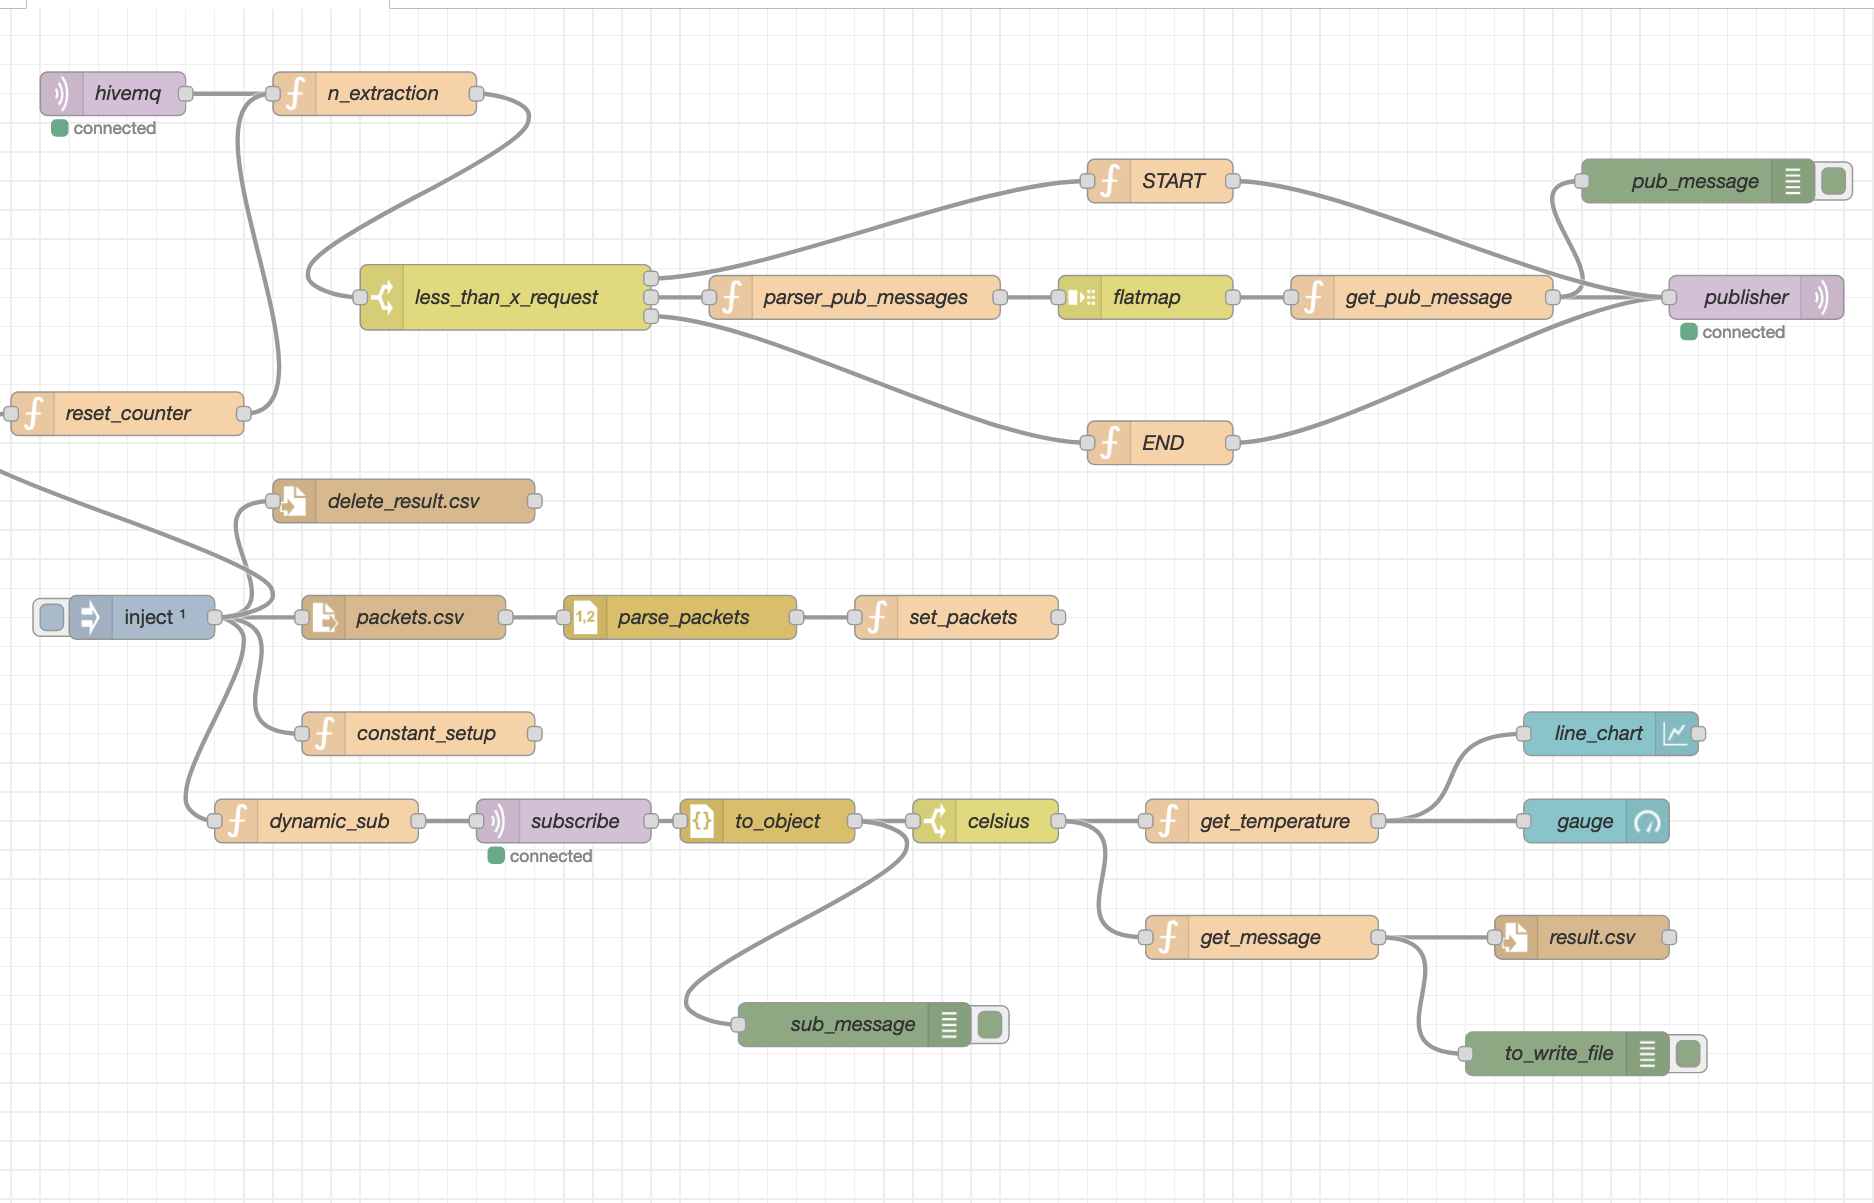
\includegraphics[scale = 0.5]{images/result.png}

\subsection*{Initialization}
Some Initialization is performed at the start of execution. Constant and \textit{packets.csv} file are imported and set as flow variables.

\subsection*{Extract the ID}
Hivemq node is the MQTT client that receives id random generated requests, which are used to first extract the \textit{n} identifier based on the rules defined
on the requirement file. Along with the extracted \textit{n}, a counter updated in the context environment is passed through the \textit{less\_than\_x} switch.
For the first request, so when the counter is one, when send a mqtt publish request with a payload containing \textit{"START"}.
If $0 < counter < max\_req == 100$, then the flow moves along the \textit{parser\_pub\_messages}, which is in charge of
finding the packet having the specified id and producing the corresponding publish messages to send later to the MQTT publisher.
The code of the parser can be seen here below, which first fetch the flow variable initialized at the start of the process by
reading the \textit{packets.csv} file. 
First we filter all the packets having the specified \textit{id} and starting with \textit{Publish Message}, then 
we leverage on two regex expression to transform topics and messages strings into array, that are flattened
into array of objects, each of them representing a publish message request to send to the broker.
These array of messages is then handled as a stream of objects and published one at a time in the MQTT client publisher.
\begin{minted}{javascript}
    const {n, id} = msg
    const packets = flow.get("packets") ?? []
    const person_code = flow.get('person_code')
    const timestamp = new Date().toISOString()
    const topic = `/polimi/iot2023/challenge2/${person_code}`

    const messages = packets.filter(r => r['No.'] == n && r['Info'].startsWith('Publish Message'))
        .map(r => {
            var { ['No.']: No, ['Info']: info, ['Message']: message, ...rest } = r;
            const regex_infos = /(?<=\[)[^\[\]]*(?=\])/g;
            const topics = info ? info.match(regex_infos) : []
            const regex_messages = /{[^}]+}/g;
            const messages = message ? message.match(regex_messages) : []
            return { ...rest, topics, messages };
        })
        .flatMap(r => {
            const res = [];
            const topic_len = r.topics ? r.topics.length : 0;
            for (let i = 0; i < topic_len; i++) {
                const {topics, messages, ...rest} = r
                res.push({ 
                    ...rest,
                    topic: topics[i], 
                    message: messages[i]
                    })
            }
            return res;
        })
        .map(p => {
            const {message} = p
            const payload = {
            'CURRENT_TIMESTAMP': timestamp,
            'PREVIOUS_ID': id,
            'MQTT_PUBLISH_PAYLOAD': message
            }
            return {topic, payload};
        })
    return {payload: messages};
\end{minted}
\captionof*{minted}{parser\_pub\_messages}


\subsection*{Subscription}
The MQTT subscriber is dynamically subscribed based on the person\_code set in the initialization phase.
Then for each message received, it is first translated into a javascript object, and passed through the 
flow if contains a celsius temperature.

\begin{center}
    \includegraphics*[scale = 0.6]{images/chart.png}
    \captionof*{images/chart.png}{Chart and gauge of the temperatures collected}
\end{center}



\section*{Nodes}
\subsection*{n\_extraction}
Logic for extractions of n, which also contains some control logic for the reset of the context variable \textit{counter}, which keeps tracks
of the number of requests handled.
\begin{minted}{javascript}
const { reset_counter = false } = msg;
if (reset_counter) {
    context.set('counter', 0);
    return;
}
const {payload} = msg;
const divider = flow.get('divider');
const person_code = flow.get('person_code');
var {id} = payload
var counter = parseInt(context.get('counter') ?? 0);
context.set('counter', ++counter)
if (!id || !divider) return;
const n = (parseInt(id) + parseInt(person_code.slice(-4))) % divider
return {n, id, counter};
\end{minted}

\subsection*{constant\_setup}
\begin{minted}{javascript}
const {payload: packets} = msg;
flow.set('person_code', "10605775");
flow.set('divider', 7711);
return msg;
\end{minted}

\subsection*{dynamic\_sub}
\begin{minted}{javascript}
const person_code = flow.get('person_code');
const topic = `/polimi/iot2023/challenge2/${person_code}`
const action = 'subscribe';
return {action, topic};
\end{minted}


\end{document}